\section{Validierung}
In diesem Kapitel geht es darum, Anforderungen und Eigenschaften des Aktor- und Sensorbausteins zu testen.
\subsection{Sensorbaustein}
\subsubsection{ESD Test}
Der Sensorbaustein wird wie eine Unterputzsteckdose verbaut und die Frontplatte dient als User-Interface. 
Genauer bedeutet es, dass der Benutzer, die Touchflächen der Frontplatte berühren muss, um mit dem Sensorbaustein zu interagieren. 
Durch das berühren kann es jedoch zu elektrostatischen Entladungen kommen, die der Sensorbaustein überstehen muss.
Deswegen wurde mithilfe eines ESD-Tests, getestet bis zu welchem Prüfschärfegrad, also bis zur welcher Entladespannung der Sensorbaustein funktioniert.
In der Tabelle \ref{tab: ESD_Testablauf} sind die Prüfschärfegrade und deren Spannungen abgebildet.
Für den Test wurde die Kontaktentladung genommen, mit welcher eine Entladung über einen Finger nachgestellt wird.\\
Der Testablauf war wie folgt \cite{schleuniger_emv_w8_2020}:\\
\\
- Beginn beim tiefsten Schärfegrad\\
- 1 Entladung/s\\
- mind. 10 Entladungen, jeweils auf jeder Touchfläche\\


\begin{figure}[H]
	\centering
	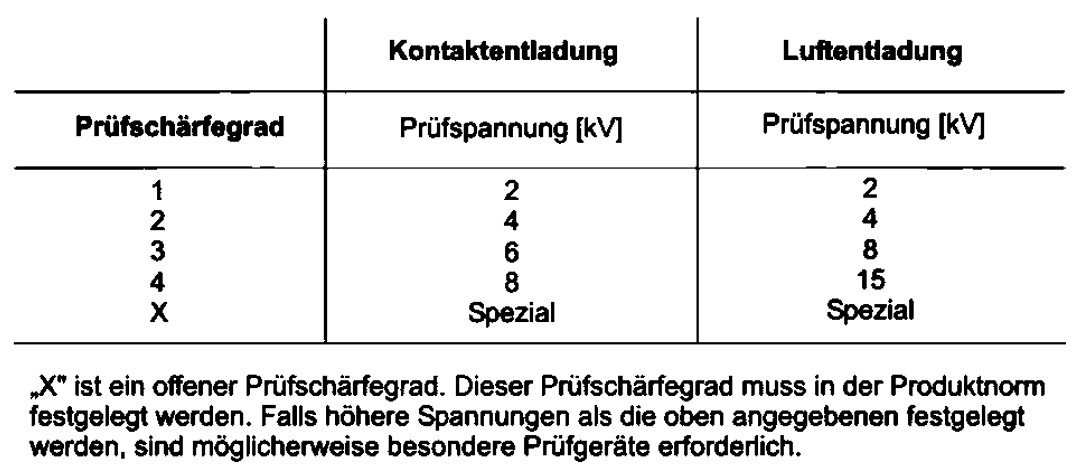
\includegraphics[width=0.8\textwidth]{graphics/ESD_Testablauf.jpg}
	\caption{ESD Testablauf \cite{schleuniger_emv_w8_2020}}
	\label{tab: ESD_Testablauf}
\end{figure}

Das Resultat war, dass der Sensorbaustein beim Prüfschärfegrad 4 Schaden nahm. Bei geringeren Spannungen war er funktionstüchtig. Was bedeutet, dass der Sensorbaustein Prüfschärfegrad 3 mit 6\,kV erreicht hat. Der Schaden beim Grad 4 war sichtbar und befand sich beim Seriell/UART-Wandler (Abbildung: \ref{pic: ESD_Schaden}), was nicht zu erwarten war. Der betroffene Pin war die Spannungsversorgung des IC's, dazu wurden direkt die 5\,V der Eingangsspeisung genommen, die Entweder über USB oder Pins angeschlossen wird. Beide Spannungsversorgungen sind miteinander verbunden, da in der Anwendung nur eines von beidem verwendet wird. Theoretisch wäre es auch möglich gewesen die 3.3\,V als Versorgung des Seriell/UART-Wandlers zu nehmen, die Frage ist, ob dann der gleiche Schaden aufgetreten wäre. Die Schutzdioden welche Über- und Unterspannung ableiten sind mit Ground bzw. 3.3\,V verbunden und nur der Seriell/UART-Wandler und der DC/DC Wandler sind an der 5\,V Speisung angeschlossen. Schlussendlich ist der Strom über den Seriell/UART-Wandler abgeflossen und hat ihn zerstört.

\begin{figure}[H]
	\centering
	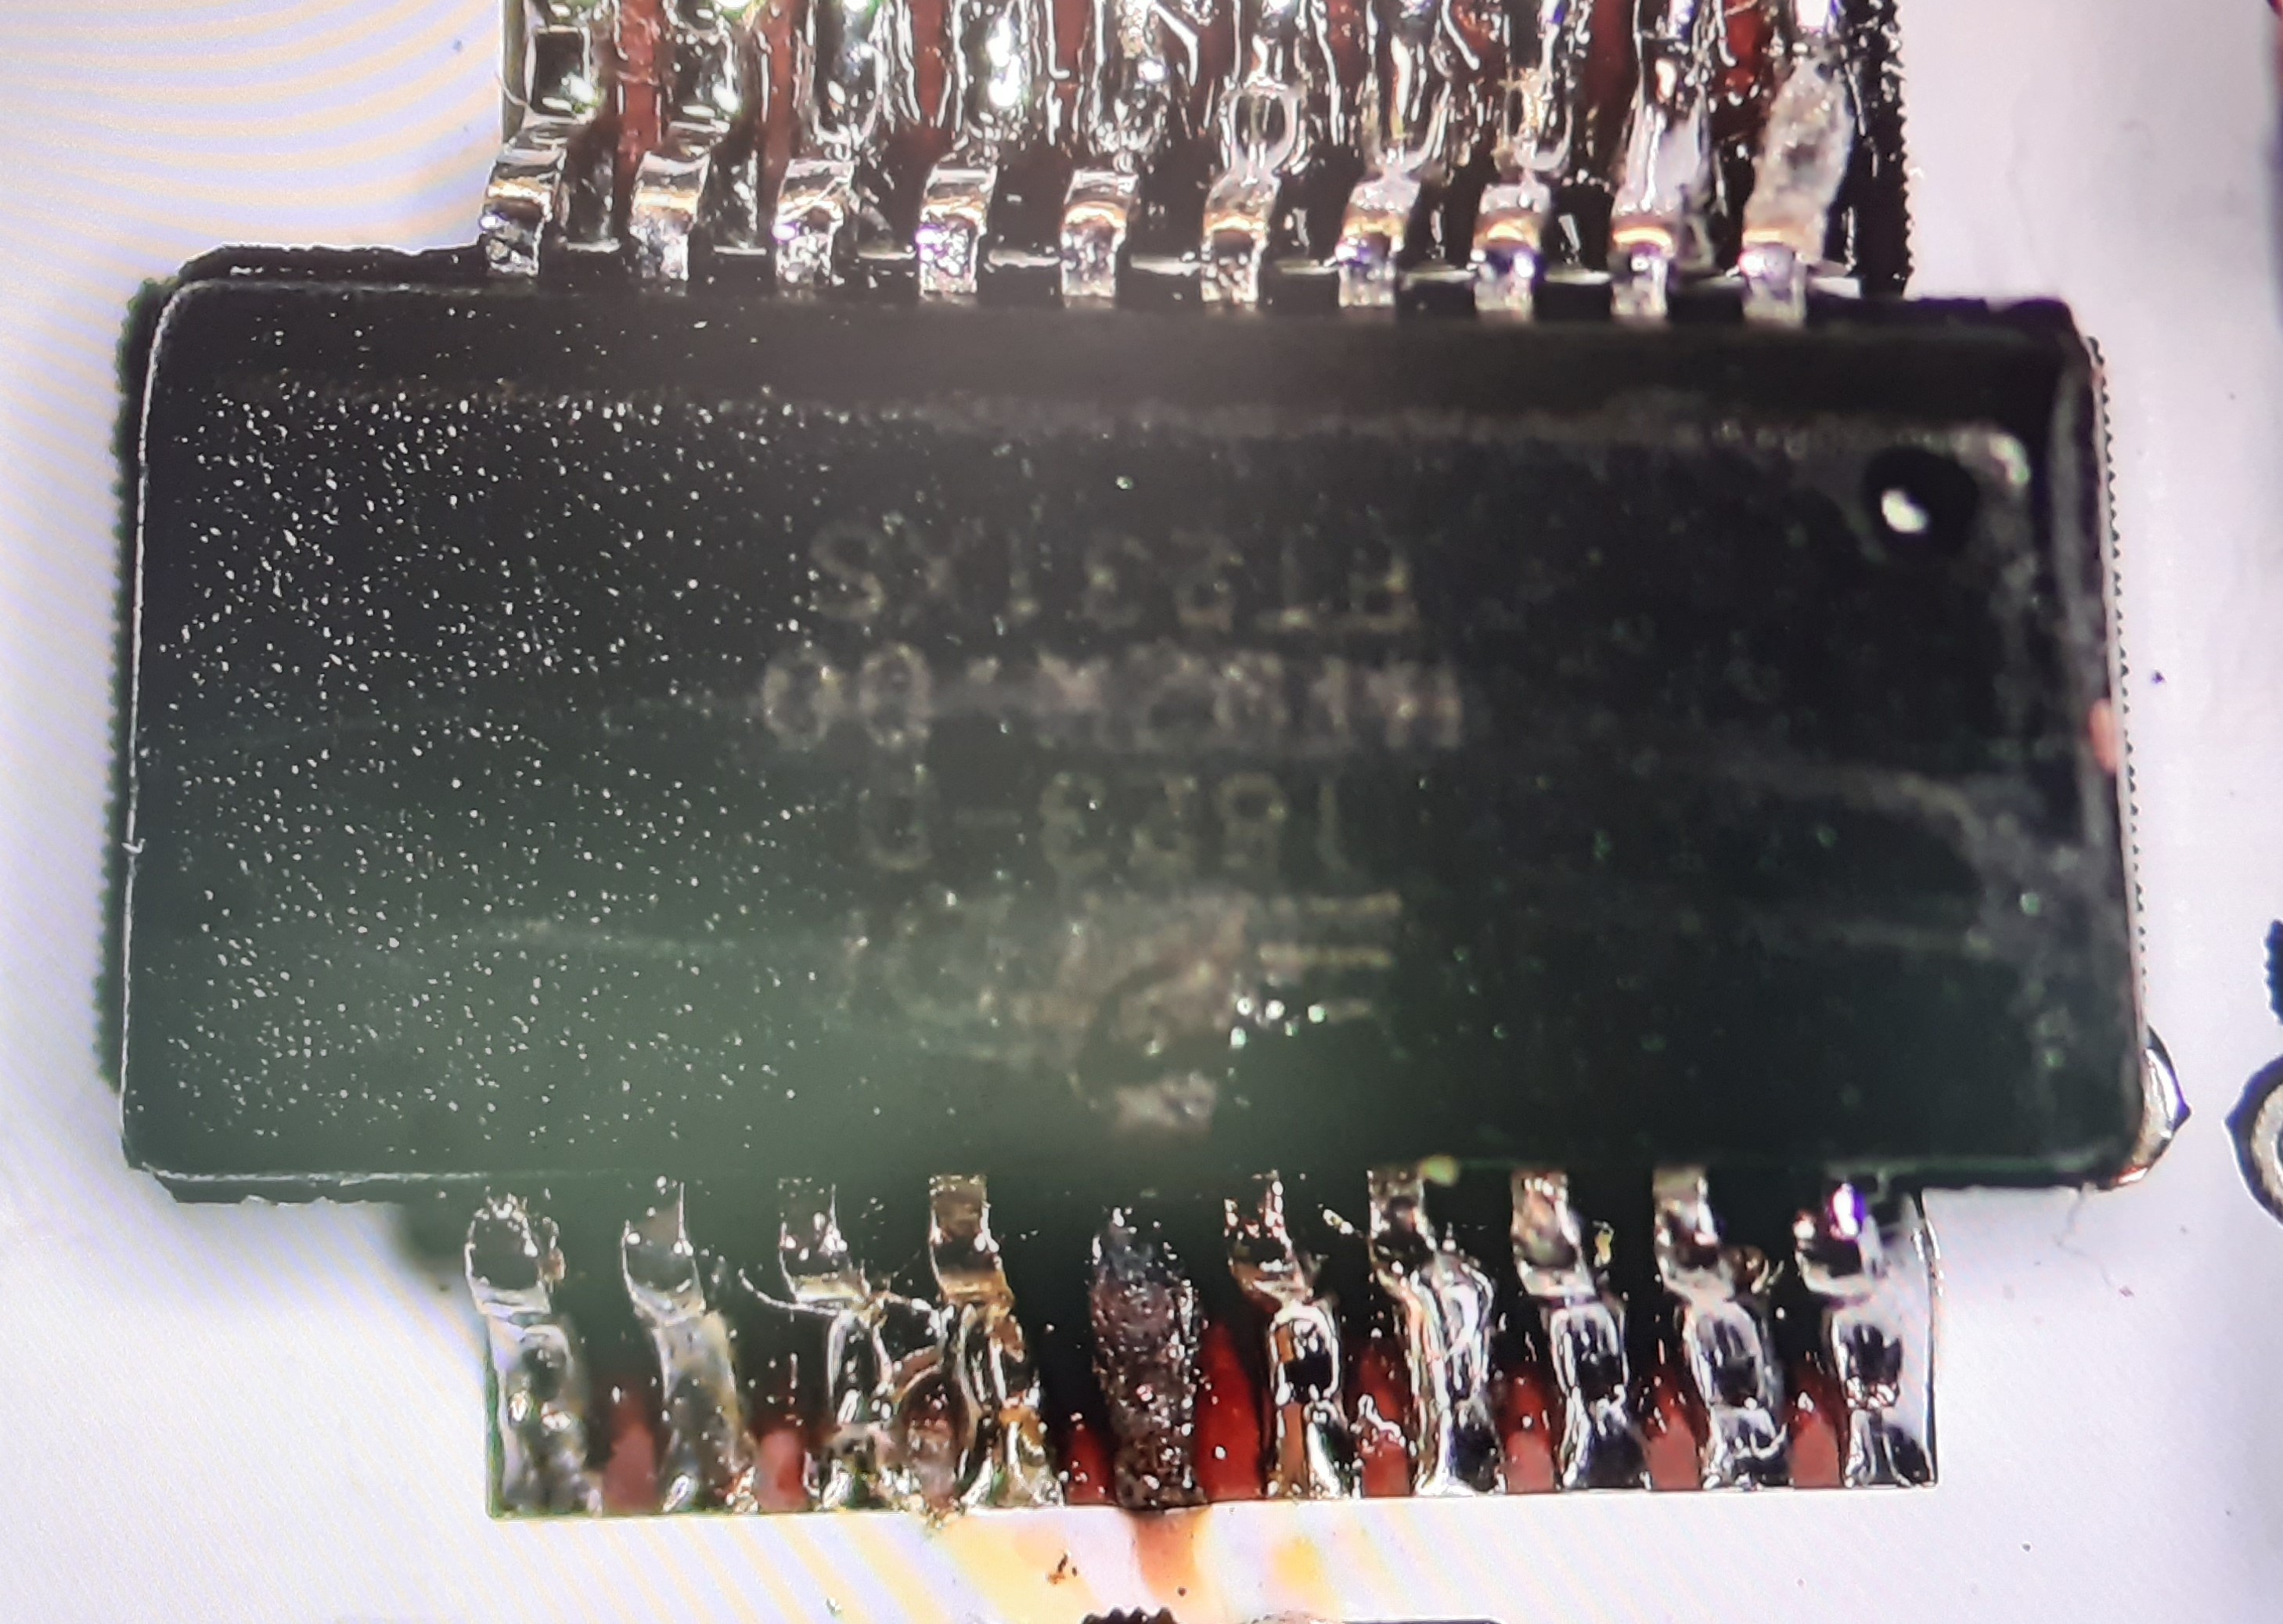
\includegraphics[width=0.8\textwidth]{graphics/ESD_Schaden.jpg}
	\caption{Der Schaden am Seriell/Uart-Wandler welcher, wegen des ESD Tests mit Prüfschärfegrad 4 zu Stande kam}
	\label{pic: ESD_Schaden}
\end{figure}

\subsubsection{Energieverbrauch des Sensorbausteins}
Der Sensorbaustein wurde unter folgenden Bedingungen gemessen:
\begin{enumerate}
	\item ungeschalteter Normalzustand (Abbildung: \ref{pic: Sensorbaustein_ungeschaltet}) \\(Der Sensorbaustein wird nicht bedient und hat eine Verbindung mit einem WLAN Netzwerk) \\
	Der Sensorbaustein hat eine mittlere Leistungsaufnahme von ca. 370\,mW. Auffällig ist, dass die Leistung mit einer Periode von 10\,s schwankt, was dem zu Programm zugrunde liegt, denn die Temperaturmessung, denn das Status LED toggelt alle 10\,s, um anzuzeigen, dass die Temperatur nach 10\,s wieder gemessen wird. Unregelmäßige Leistungssprünge von bis zu ca. 400\,mW kommen häufiger vor, was wahrscheinlich durch das WLAN ausgelöst wird.
	\\
	\item geschalteter Normalzustand (Abbildung: \ref{pic: Sensorbaustein_geschaltet})\\ (Der Sensorbaustein wird bedient und hat eine Verbindung mit einem WLAN Netzwerk)\\
	In den Zeiten um ca. 35\,s, 60\,s und 85\,s werden alle Vier Taster betätigt, die Leistungsaufnahme steigt um 10\,mW von vorher 370\,mW auf ca. 380\,mW, was vertretbar ist.
	\\
	\item Keine Verbindung (Abbildung: \ref{pic: Sensorbaustein_keine_Verbindung})\\ (Der Sensorbaustein findet kein zulässiges WLAN Netzwerk)\\
	In diesem Zustand hat der Sensorbaustein eine mittlere Leistungsaufnahme von 930\,mW, was beträchtlich ist. Dies ist daran geschuldet, dass der Sensorbaustein vermutlich seine seine Signalstärke erhöht, um ein Netzwerk zu finden. Deswegen wird nicht empfohlen, den Sensorbaustein, in diesem Zustand zu lassen.
\end{enumerate}


\begin{figure}[H]
	\centering
	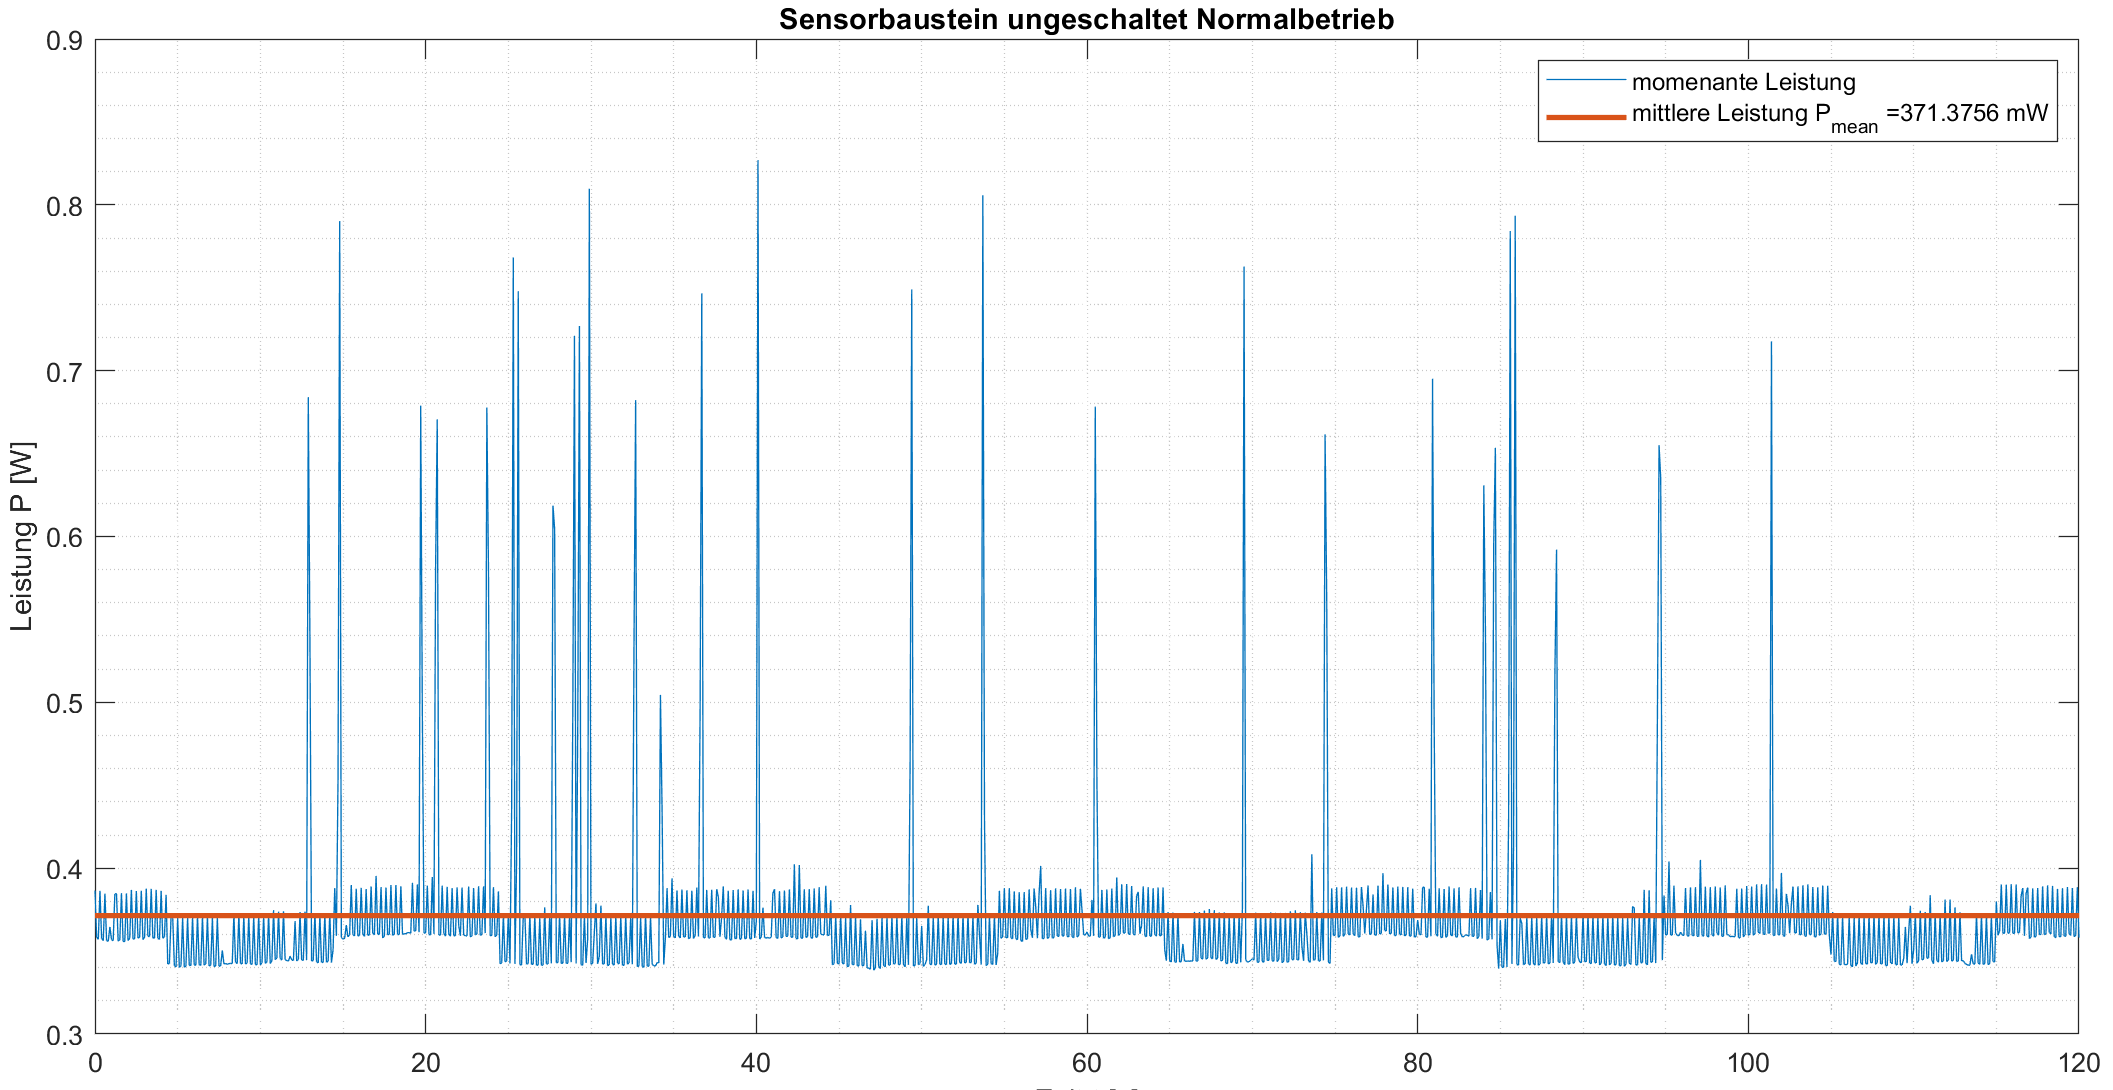
\includegraphics[width=1\textwidth]{graphics/Sensorbaustein_ungeschaltet.png}
	\caption{Die Leistung des Sensorbausteins, wenn er nicht bedient wird und mit dem Netzwerk verbunden ist}
	\label{pic: Sensorbaustein_ungeschaltet}
\end{figure}

\begin{figure}[H]
	\centering
	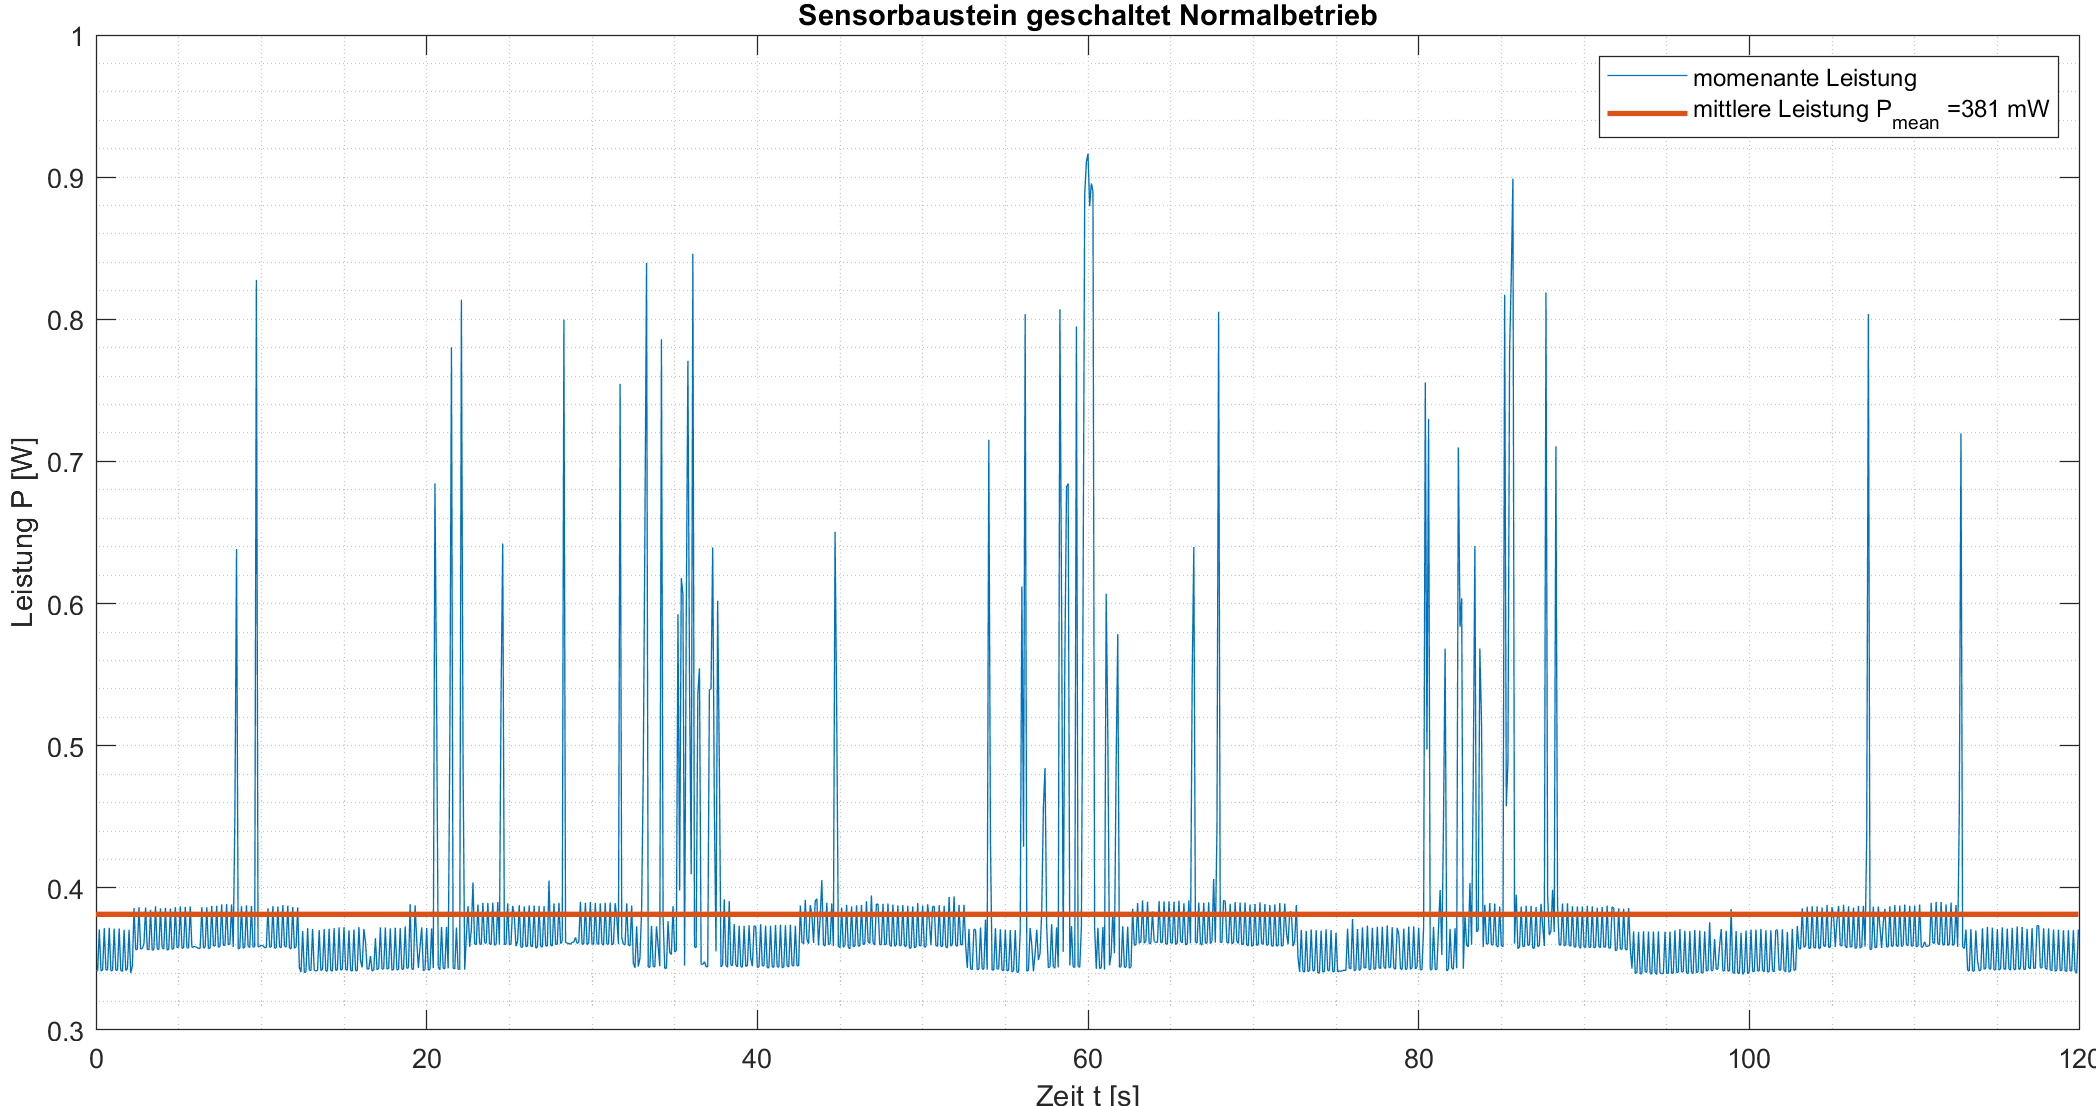
\includegraphics[width=1\textwidth]{graphics/Sensorbaustein_geschaltet.png}
	\caption{Die Leistung des Sensorbausteins, wenn er bedient wird und mit dem Netzwerk verbunden ist}
	\label{pic: Sensorbaustein_geschaltet}
\end{figure}

\begin{figure}[H]
	\centering
	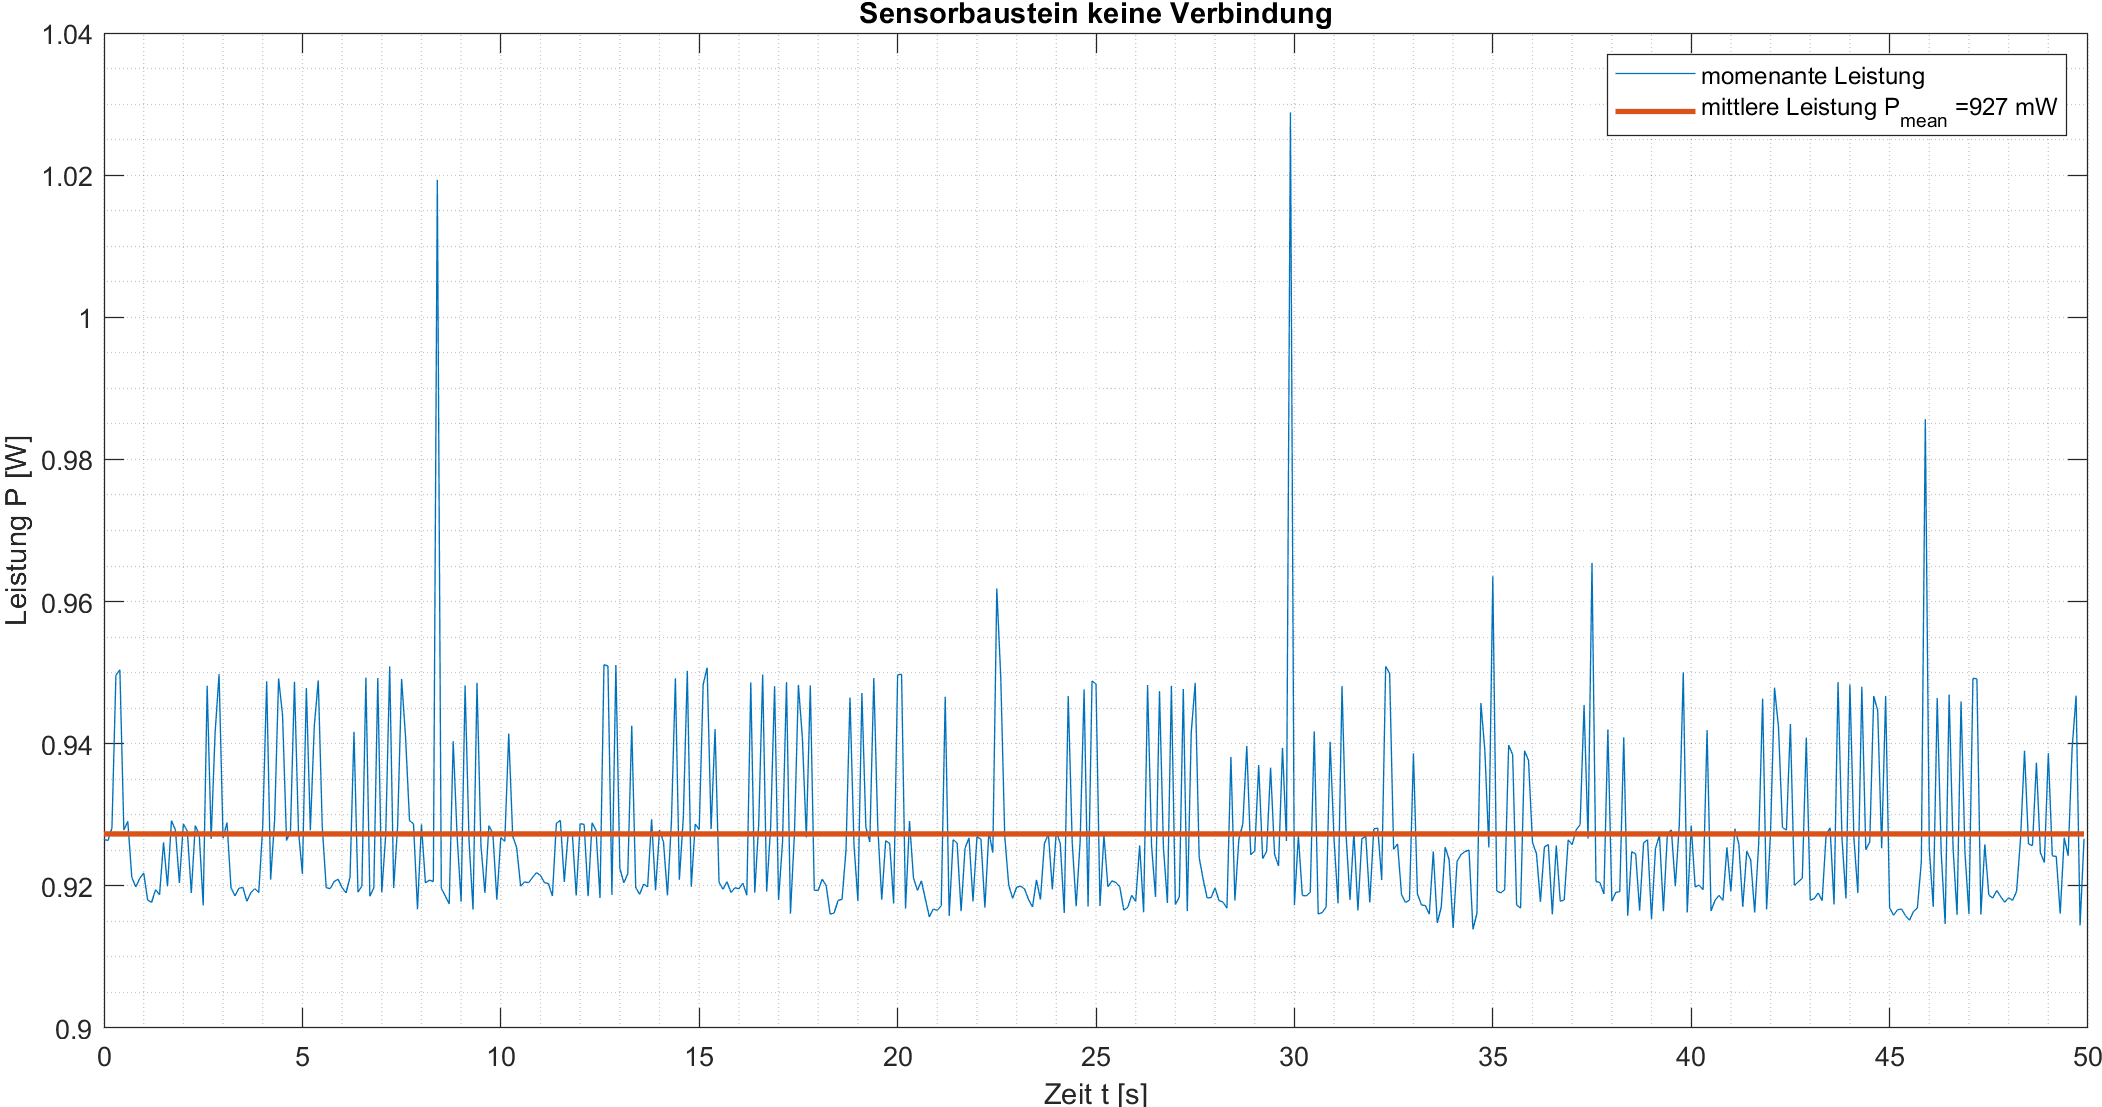
\includegraphics[width=1\textwidth]{graphics/Sensorbaustein_keine_Verbindung.png}
	\caption{Die Leistung des Sensorbausteins, wenn er einen Verbindungsaufbau versucht, aber kein geeignetes WLAN Netzwerk vorhanden ist}
	\label{pic: Sensorbaustein_keine_Verbindung}
\end{figure}




\subsubsection{Temperaturmessung}
Es wird berechnet, wie gross die Abweichung der Temperaturmessung sein kann. Dazu wurde mit $U_\text{ref} = 2.39\,V$ und einer Temperatur von -4.6\,°C $\approx$ 5\,°C  gerechnet (folglich Kapitel \ref{tempf}), diese Temperatur wurde als untere Grenze genommen und sie wird die Abweichung im gewählten Temperaturbereich maximieren, folglich Gleichung \ref{eq: dRT}. Gerechnet wird mit einem Vorwiderstand $R_{\text{V}}$ von $100\,k\Omega$ mit 1\,\% Abweichung und einem NTC mit einem Widerstand von $R_{\text{T}}$, welcher 5\,\% Abweichung hat.
\\
Werte:
\begin{align*}
R_{T,4.6} &= 481\,k\Omega\\
R_{T,max} &= 481\,k\Omega \cdot 1.05 = 505\,k\Omega\\
R_{T,20.2} &= 126\,k\Omega\\
R_{T,20.2,max} &= 126\,k\Omega \cdot 1.05 = 132\,k\Omega\\
R_V &= 100\,k\Omega\\
R_{V,min} &= 100\,\Omega \cdot 0.99 = 99k\,\Omega\\
B &= 4250\,K\\
T_{25} &= 298.15\,K\\
\end{align*}
\\
Was als erhöhte Spannung an $U_{ntc}$ bei -4.6°C anliegen würde:
\begin{align}
U_{ntc,max} &= U_{\text{ref}} \cdot \frac{R_{T,max}}{R_{T,max}\;+\;R_{V,min}} = 2.39\;V \cdot \frac{ 505\,k\Omega}{(505\,k\Omega\;+\;99\,k\Omega)} = 2.00\,V\label{eq: U_{ntc,max}} \\
\end{align}
\\
Was als erhöhte Spannung an $U_{ntc}$ bei 20.2°C anliegen würde:
\begin{align}
U_{ntc,max} &= U_{\text{ref}} \cdot \frac{R_{T,max}}{R_{T,max}\;+\;R_{V,min}} = 2.39\;V \cdot \frac{ 132\,k\Omega}{(132\,k\Omega\;+\;99\,k\Omega)} = 1.37\,V\label{eq: U_{ntc,20.2,max}}
\end{align}
\\
Temperatur Berechnung bei -4.6°C im Mikrocontroller:
\begin{align}
\frac{R_T}{R_V}_{max} &= \frac{U_{ntc,max}}{U_{ref}\;-\;U_{ntc,max}} = 5.13\\
T &= \frac{1}{\frac{1}{T_{25}}+\frac{1}{B} \cdot ln(\frac{R_T}{R_V}_{max})} = 267.46\,K = -5.68\,^\circ C\\
\Delta T_{max} &= -4.6^\circ C - (-5.7^\circ C) = 1.1\,K
\end{align}
\\
Temperatur Berechnung bei 20.2°C im Mikrocontroller:
\begin{align}
\frac{R_T}{R_V}_{max} &= \frac{U_{ntc,max}}{U_{ref}\;-\;U_{ntc,max}} = 1.34\\
T &= \frac{1}{\frac{1}{T_{25}}+\frac{1}{B} \cdot ln(\frac{R_T}{R_V}_{max})} = 267.46\,K = -5.68\,^\circ C\\
\Delta T_{max} &= -4.6^\circ C - (-5.7^\circ C) = 1.1\,K
\end{align}w






